%%%%%%%%%%%%%%%%%%%%%%%%%%%%%%%%%%%%%%%%%
% Jacobs Landscape Poster
% LaTeX Template
% Version 1.0 (29/03/13)
%
% Created by:
% Computational Physics and Biophysics Group, Jacobs University
% https://teamwork.jacobs-university.de:8443/confluence/display/CoPandBiG/LaTeX+Poster
% 
% Further modified by:
% Nathaniel Johnston (nathaniel@njohnston.ca)
%
% This template has been downloaded from:
% http://www.LaTeXTemplates.com
%
% License:
% CC BY-NC-SA 3.0 (http://creativecommons.org/licenses/by-nc-sa/3.0/)
%
%%%%%%%%%%%%%%%%%%%%%%%%%%%%%%%%%%%%%%%%%

%----------------------------------------------------------------------------------------
%	PACKAGES AND OTHER DOCUMENT CONFIGURATIONS
%----------------------------------------------------------------------------------------

\documentclass[final]{beamer}

\usepackage{subcaption}

\usepackage[scale=1.1, size=a0]{beamerposter} % Use the beamerposter package for laying out the poster
\usepackage[utf8]{inputenc}

\usetheme{confposter} % Use the confposter theme supplied with this template

%-----------------------------------------------------------
% Define the column widths and overall poster size
% To set effective sepwid, onecolwid and twocolwid values, first choose how many columns you want and how much separation you want between columns
% In this template, the separation width chosen is 0.024 of the paper width and a 4-column layout
% onecolwid should therefore be (1-(# of columns+1)*sepwid)/# of columns e.g. (1-(4+1)*0.024)/4 = 0.22
% Set twocolwid to be (2*onecolwid)+sepwid = 0.464
% Set threecolwid to be (3*onecolwid)+2*sepwid = 0.708

\newlength{\sepwid}
\newlength{\onecolwid}
\newlength{\twocolwid}
\newlength{\threecolwid}
\setlength{\paperwidth}{48in} % A0 width: 46.8in
\setlength{\paperheight}{36in} % A0 height: 33.1in
\setlength{\sepwid}{0.024\paperwidth} % Separation width (white space) between columns
\setlength{\onecolwid}{0.22\paperwidth} % Width of one column
\setlength{\twocolwid}{0.464\paperwidth} % Width of two columns
\setlength{\threecolwid}{0.708\paperwidth} % Width of three columns
\setlength{\topmargin}{-0.5in} % Reduce the top margin size
%-----------------------------------------------------------
\renewcommand{\figurename}{Fig.}

\definecolor{dorado}{RGB}{255,204,102}

\usepackage{graphicx}  % Required for including images

\usepackage{booktabs} % Top and bottom rules for tables

%----------------------------------------------------------------------------------------
%	TITLE SECTION 
%----------------------------------------------------------------------------------------

\title{CNN pre-training using convolutional autoencoders} % Poster title

\author{Russell Hofmann, Sabbir Ahmed, Maximilian Kohlbrenner } % Author(s)

\institute{TU Berlin} % Institution(s)

%----------------------------------------------------------------------------------------

\begin{document}

\setbeamercolor{block title}{fg=ngreen,bg=white} % Colors of the block titles
\setbeamercolor{block body}{fg=black,bg=white} % Colors of the body of blocks
\setbeamercolor{block alerted title}{fg=black, bg=gray} % Colors of the highlighted block titles
\setbeamercolor{block alerted body}{fg=black, bg=white} % Colors of the body of highlighted blocks


\addtobeamertemplate{block end}{}{\vspace*{2ex}} % White space under blocks
\addtobeamertemplate{block alerted end}{}{\vspace*{2ex}} % White space under highlighted (alert) blocks

\setlength{\belowcaptionskip}{2ex} % White space under figures
\setlength\belowdisplayshortskip{2ex} % White space under equations

\captionsetup{labelformat=simple, format=hang}

\begin{frame}[t] % The whole poster is enclosed in one beamer frame

\begin{columns}[t] % The whole poster consists of three major columns, the second of which is split into two columns twice - the [t] option aligns each column's content to the top

\begin{column}{\sepwid}\end{column} % Empty spacer column

\begin{column}{\onecolwid} % The first column

%----------------------------------------------------------------------------------------
%	OBJECTIVES
%----------------------------------------------------------------------------------------

\begin{alertblock}{Setup}

\begin{block}{Experimental setup}

\begin{figure}
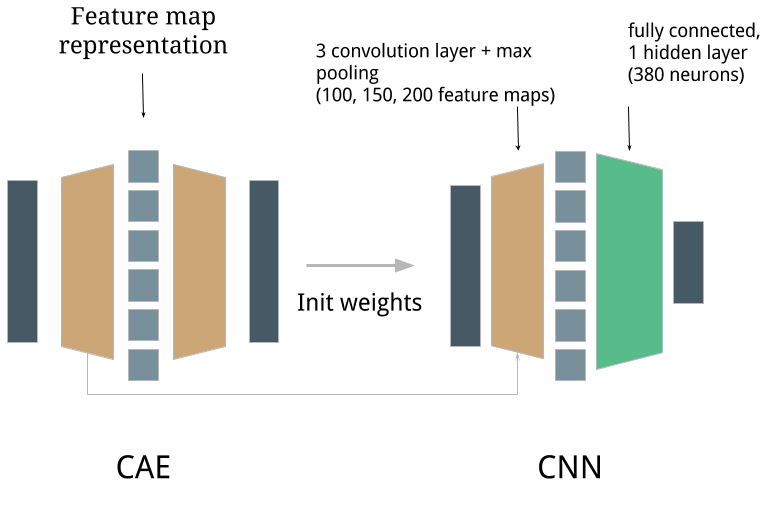
\includegraphics[width=0.8\linewidth]{graphics/setup.png}
\caption{Pre-training setup}
\end{figure}

\end{block}

\begin{block}{Convolutional Autoencoders}

\begin{itemize}
	\item convolutional architecture, reconstruction similar to deconvolution method 
	\item regularization achieved using max-pooling
\end{itemize}

\begin{figure}

\captionsetup{format=default}

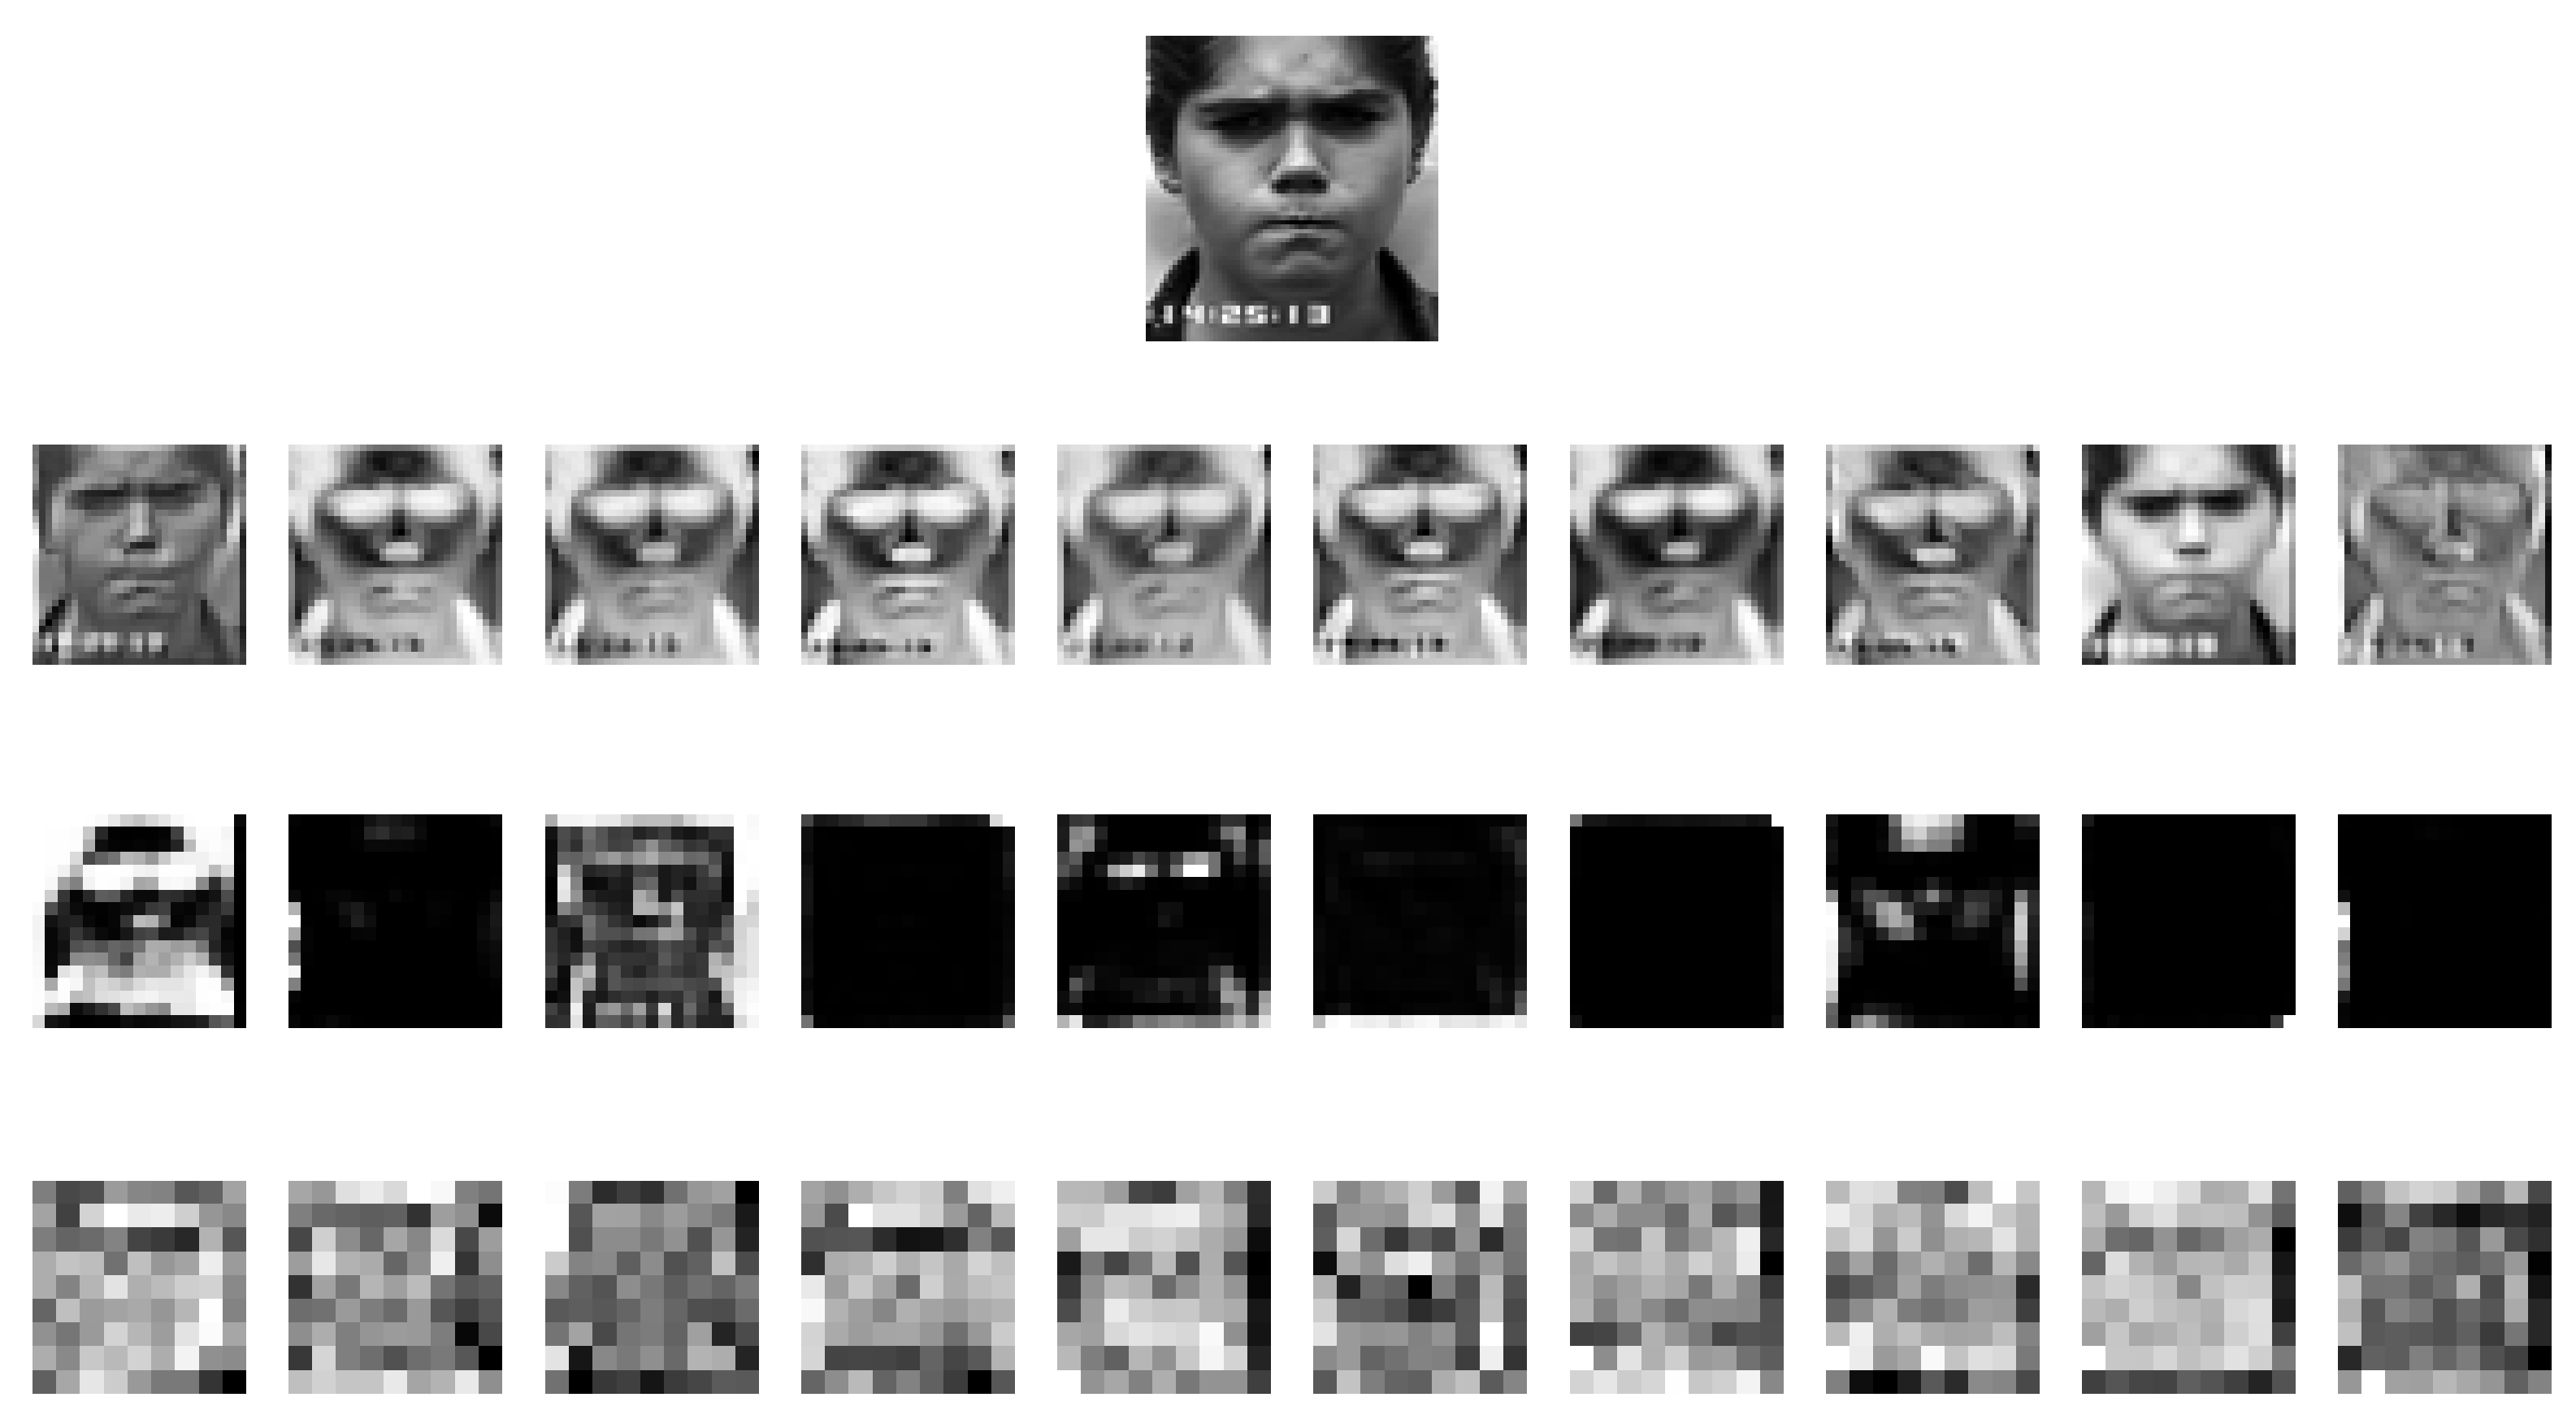
\includegraphics[width=0.8\linewidth]{graphics/feature_map_walkthrough_ckplus.png}
\caption{Input (first row), and a selection of feature maps from the subsequent convolutional layers (rows 2,3 and 4). The last row (feature maps for the 3rd convolution layer) makes up the hidden representation of the CAE}
\end{figure}

\end{block}

\begin{block}{CAE: Activation and Error Function}
	\centering
	%\textbf{Activation and Error Function}
	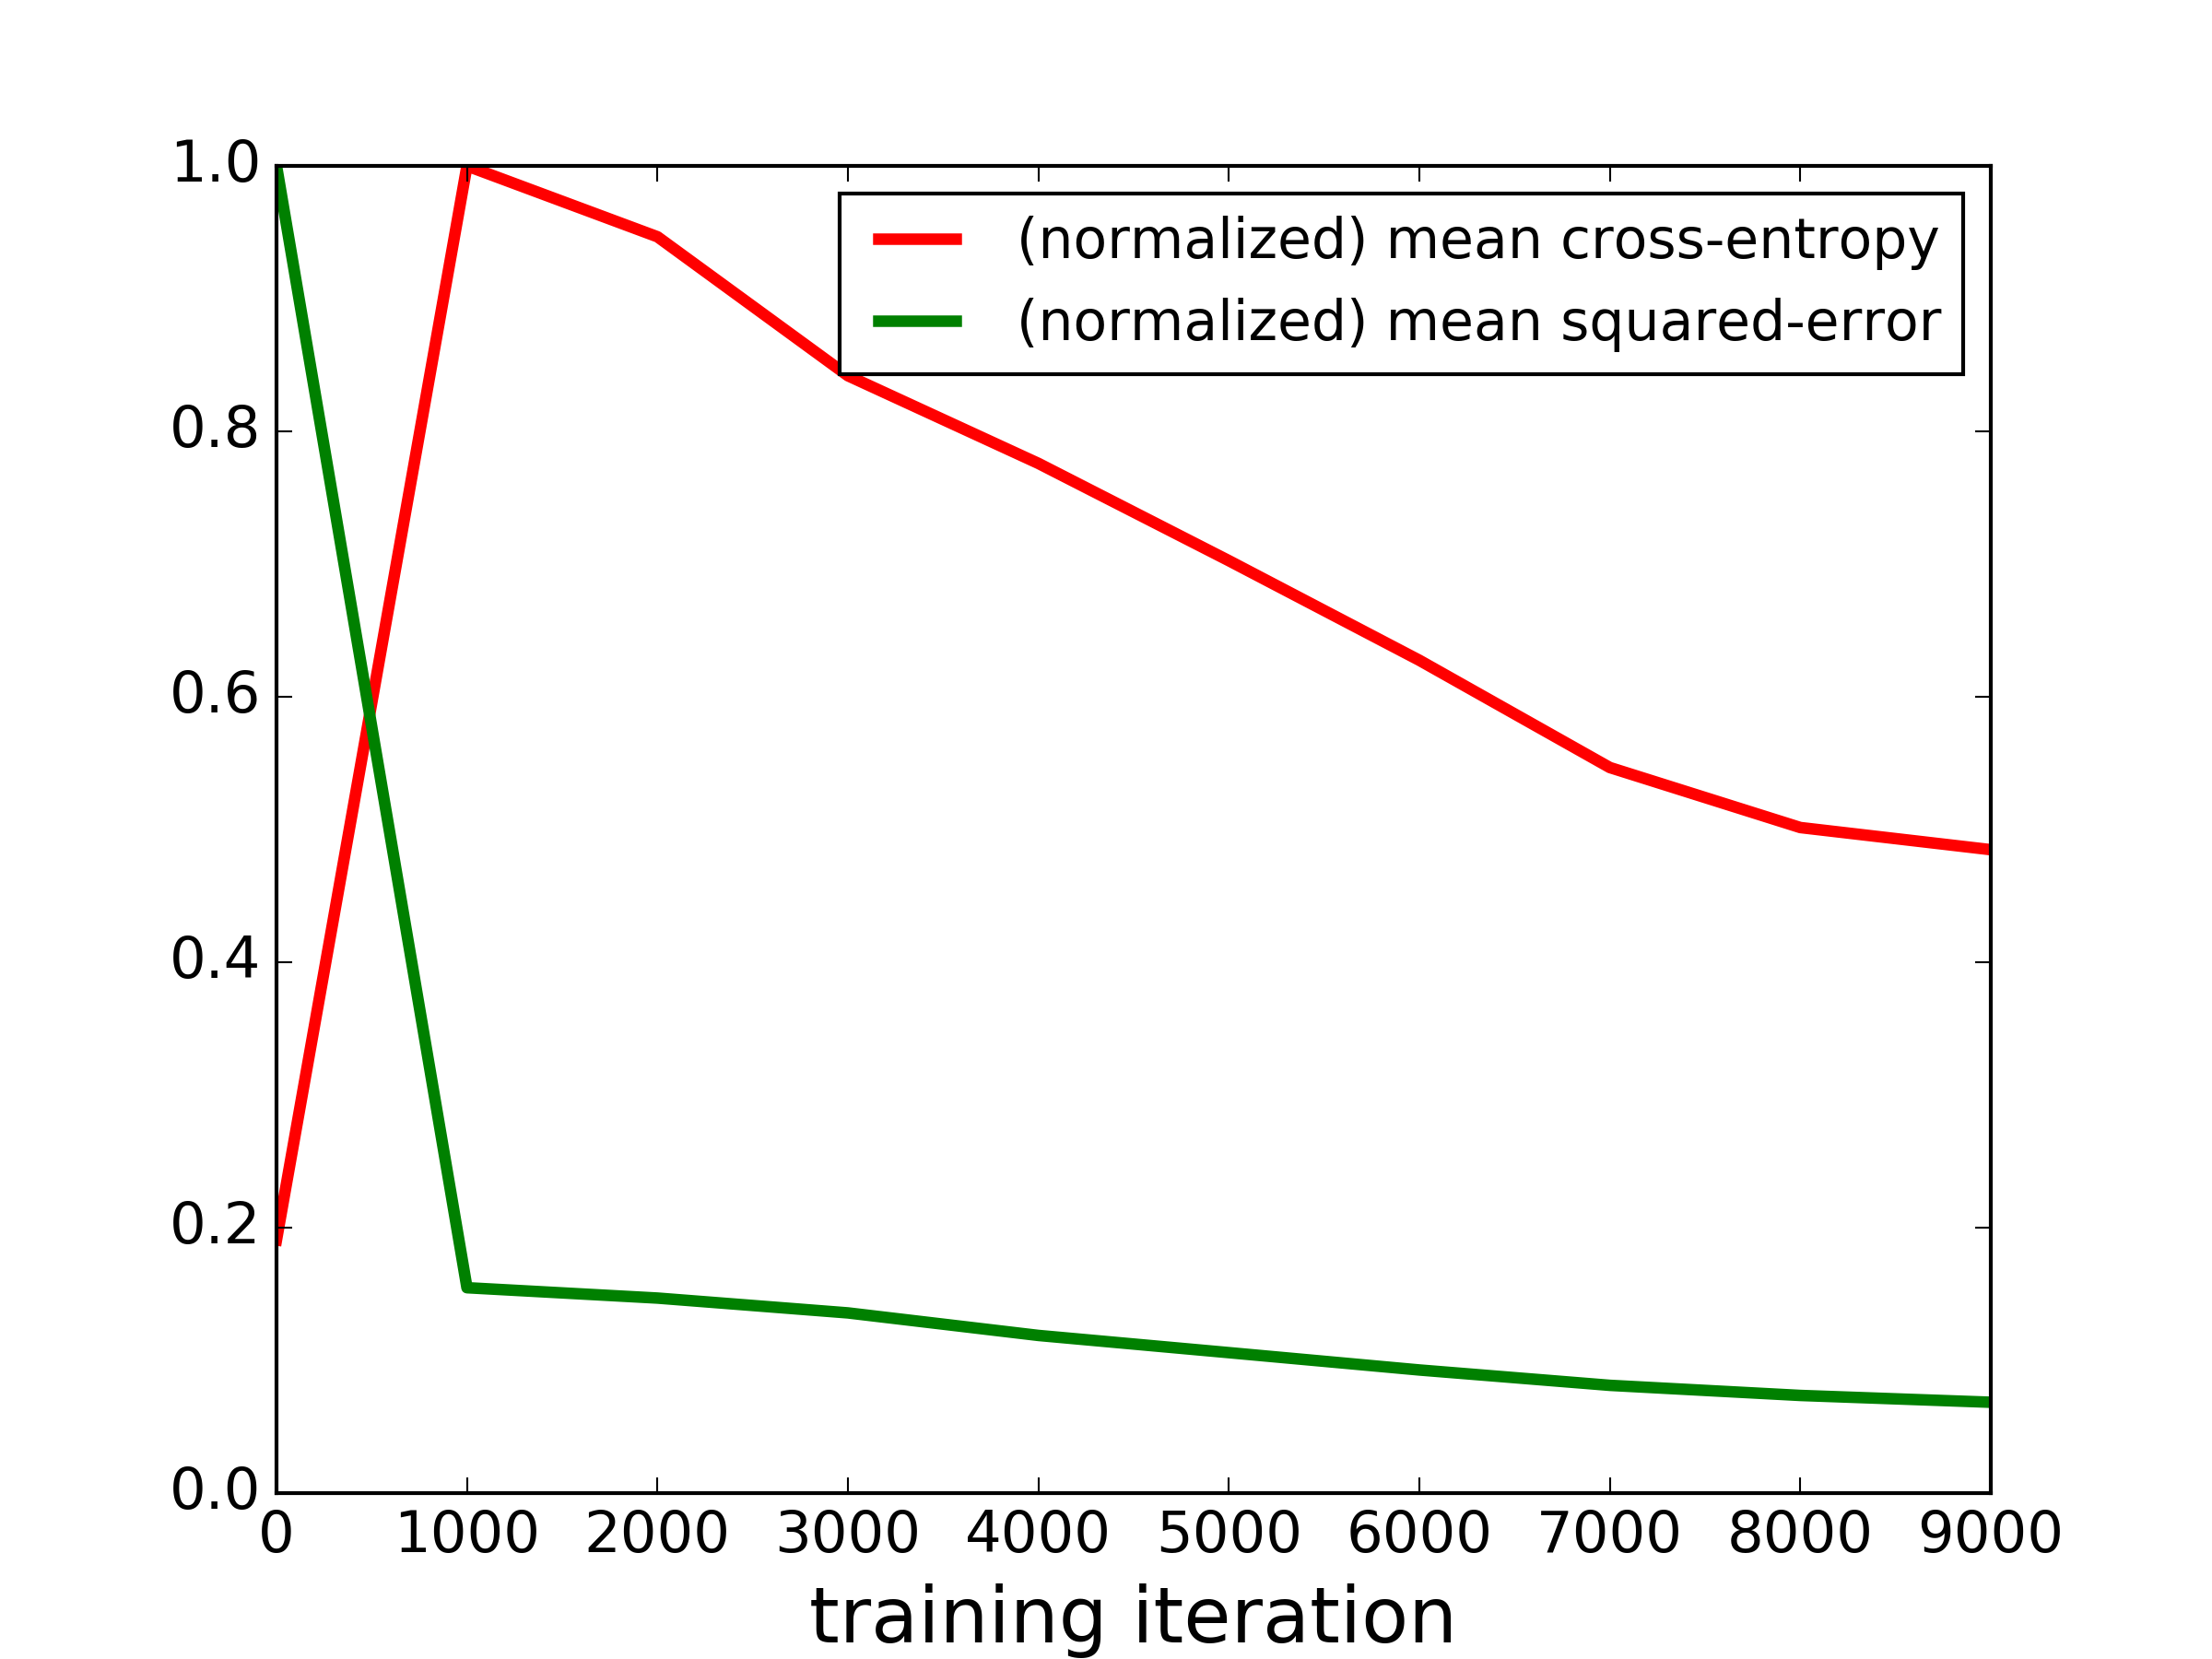
\includegraphics[width=.7\linewidth]{graphics/mse_ce_comparison.png}

	\begin{itemize}
		\item Activation function: scaled tanh (saturating, sigmoidal)
		\item Error function     : mean-squared error (mean cross-entropy produced blank reconstruction)
	\end{itemize}

\end{block}


\end{alertblock}

%----------------------------------------------------------------------------------------
%	INTRODUCTION
%----------------------------------------------------------------------------------------

\end{column} % End of the first column

% ----------------------------------------------
% SECOND COLUMN
% ----------------------------------------------

\begin{column}{\sepwid}\end{column} % Empty spacer column


\begin{column}{\threecolwid}


\begin{alertblock}{Pre-Training Experiments}

\centering

\begin{columns}[t, totalwidth=0.9\threecolwid] % Split up the two columns wide column

	%\begin{column}{\onecolwid}\vspace{-.6in} % The first column within column 2 (column 2.1)



	\begin{column}{0.9\onecolwid} % Begin a column which is one column wide (subcolumn 1)
	\begin{block}{MNIST}

	\begin{figure}

	\centering
	
\includegraphics[width=0.2\linewidth]{graphics/reconstructions/mnist/input_00.png}
	
\includegraphics[width=0.2\linewidth]{graphics/reconstructions/mnist/input_01.png}
	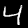
\includegraphics[width=0.2\linewidth]{graphics/reconstructions/mnist/input_02.png}

	
\includegraphics[width=0.2\linewidth]{graphics/reconstructions/mnist/reconstruction_00.png}
	
\includegraphics[width=0.2\linewidth]{graphics/reconstructions/mnist/reconstruction_01.png}
	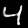
\includegraphics[width=0.2\linewidth]{graphics/reconstructions/mnist/reconstruction_02.png}


	\caption{\emph{MNIST} example images (top) and CAE reconstructions (bottom)}

	\end{figure}

	\emph{Dataset Characteristics:}

	\begin{itemize}
		\item Comparatively simple (linear classifier achieves > 90\% accuracy)
	\end{itemize}

	\end{block}
	\end{column}

	\begin{column}{0.9\onecolwid}
	\begin{block}{CIFAR-10}
	\begin{figure}
	\centering
	%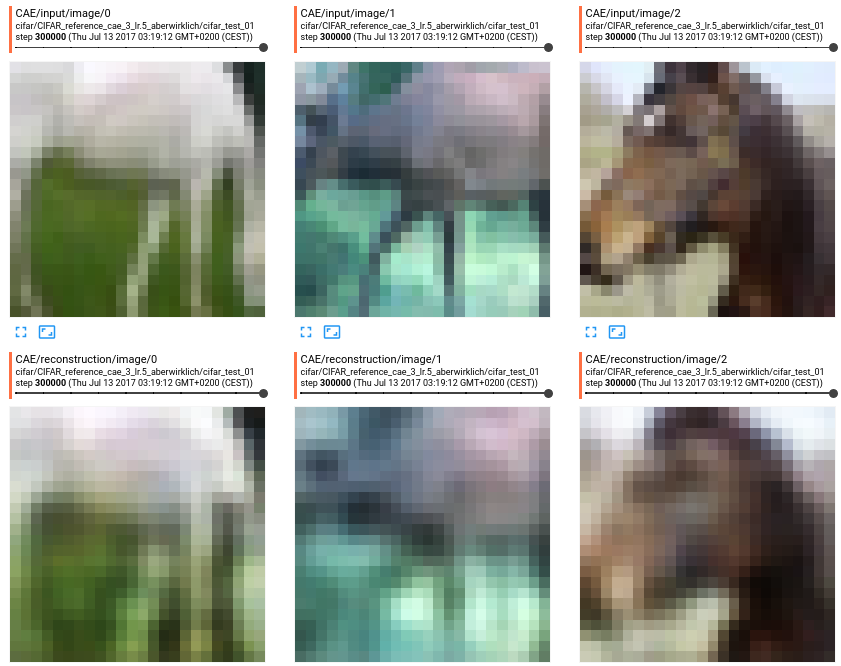
\includegraphics[width=0.8\linewidth]{graphics/cifar_reconstructions.png}
	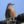
\includegraphics[width=0.2\linewidth]{graphics/reconstructions/cifar/input_00.png}
	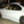
\includegraphics[width=0.2\linewidth]{graphics/reconstructions/cifar/input_01.png}
	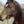
\includegraphics[width=0.2\linewidth]{graphics/reconstructions/cifar/input_02.png}

	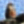
\includegraphics[width=0.2\linewidth]{graphics/reconstructions/cifar/reconstruction_00.png}
	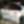
\includegraphics[width=0.2\linewidth]{graphics/reconstructions/cifar/reconstruction_01.png}
	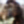
\includegraphics[width=0.2\linewidth]{graphics/reconstructions/cifar/reconstruction_02.png}

	\caption{\emph{CIFAR-10} example images(top) and CAE reconstructions(bottom)}

	\end{figure}

	\emph{Dataset Characteristics:}\\
	\begin{itemize}
	\item natural image classification (difficult)
	\item comparably low resolution
	\end{itemize}
	\end{block}
	\end{column}

	\begin{column}{0.9\onecolwid}
	\begin{block}{Extended Cohn-Kanade (CK+)}

	\begin{figure}
	\centering
	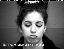
\includegraphics[width=0.2\linewidth]{graphics/reconstructions/ckplus/input_00.png}
	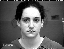
\includegraphics[width=0.2\linewidth]{graphics/reconstructions/ckplus/input_01.png}
	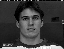
\includegraphics[width=0.2\linewidth]{graphics/reconstructions/ckplus/input_02.png}

	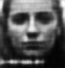
\includegraphics[width=0.2\linewidth]{graphics/reconstructions/ckplus/reconstruction_00.png}
	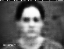
\includegraphics[width=0.2\linewidth]{graphics/reconstructions/ckplus/reconstruction_01.png}
	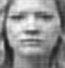
\includegraphics[width=0.2\linewidth]{graphics/reconstructions/ckplus/reconstruction_02.png}

	%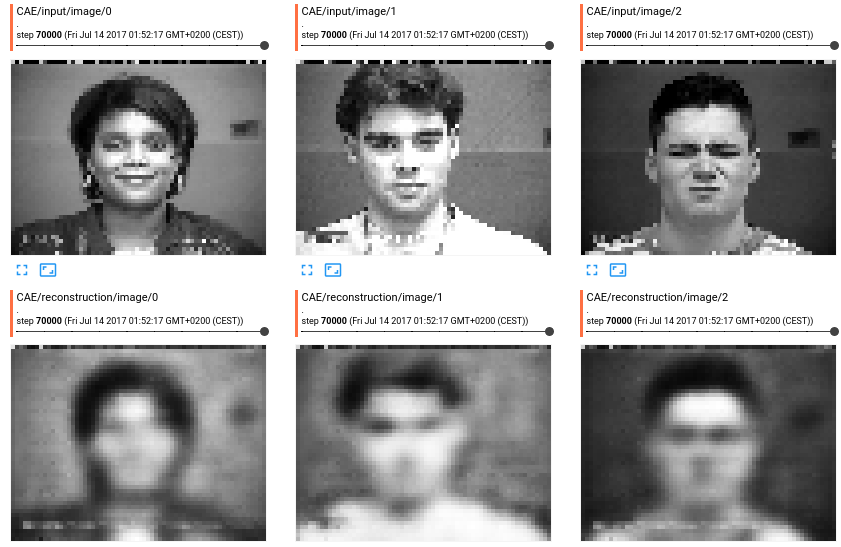
\includegraphics[width=0.8\linewidth]{graphics/ckplus_reconstructions_better.png}
	\caption{CK+ input image (top) and reconstruction (bottom)}
	\end{figure}

	\emph{Dataset Characteristics:}\\
	\begin{itemize} 
		\item pre-processing and set splitting %: image sequences, choose images and subjects and split datasets, cropping and downsampling
		\item very few data (696 train, 87 validation, 198 test in our case)
	\end{itemize}
	%\item Natural images (high resolution)
	%\item More restrained problem than CIFAR (emotion classification).
	%\item Very few datapoints 
	%\item No pre-defined splits
	%\end{itemize}

	\end{block}

	\end{column}

\end{columns}


\begin{columns}[t, totalwidth=0.9\threecolwid] % Split up the two columns wide column

	%\begin{column}{\onecolwid}\vspace{-.6in} % The first column within column 2 (column 2.1)

	\begin{column}{0.9\onecolwid} % Begin a column which is one column wide (subcolumn 1)
	\begin{block}{}
	\emph{Experimental results:}

	\begin{figure}
	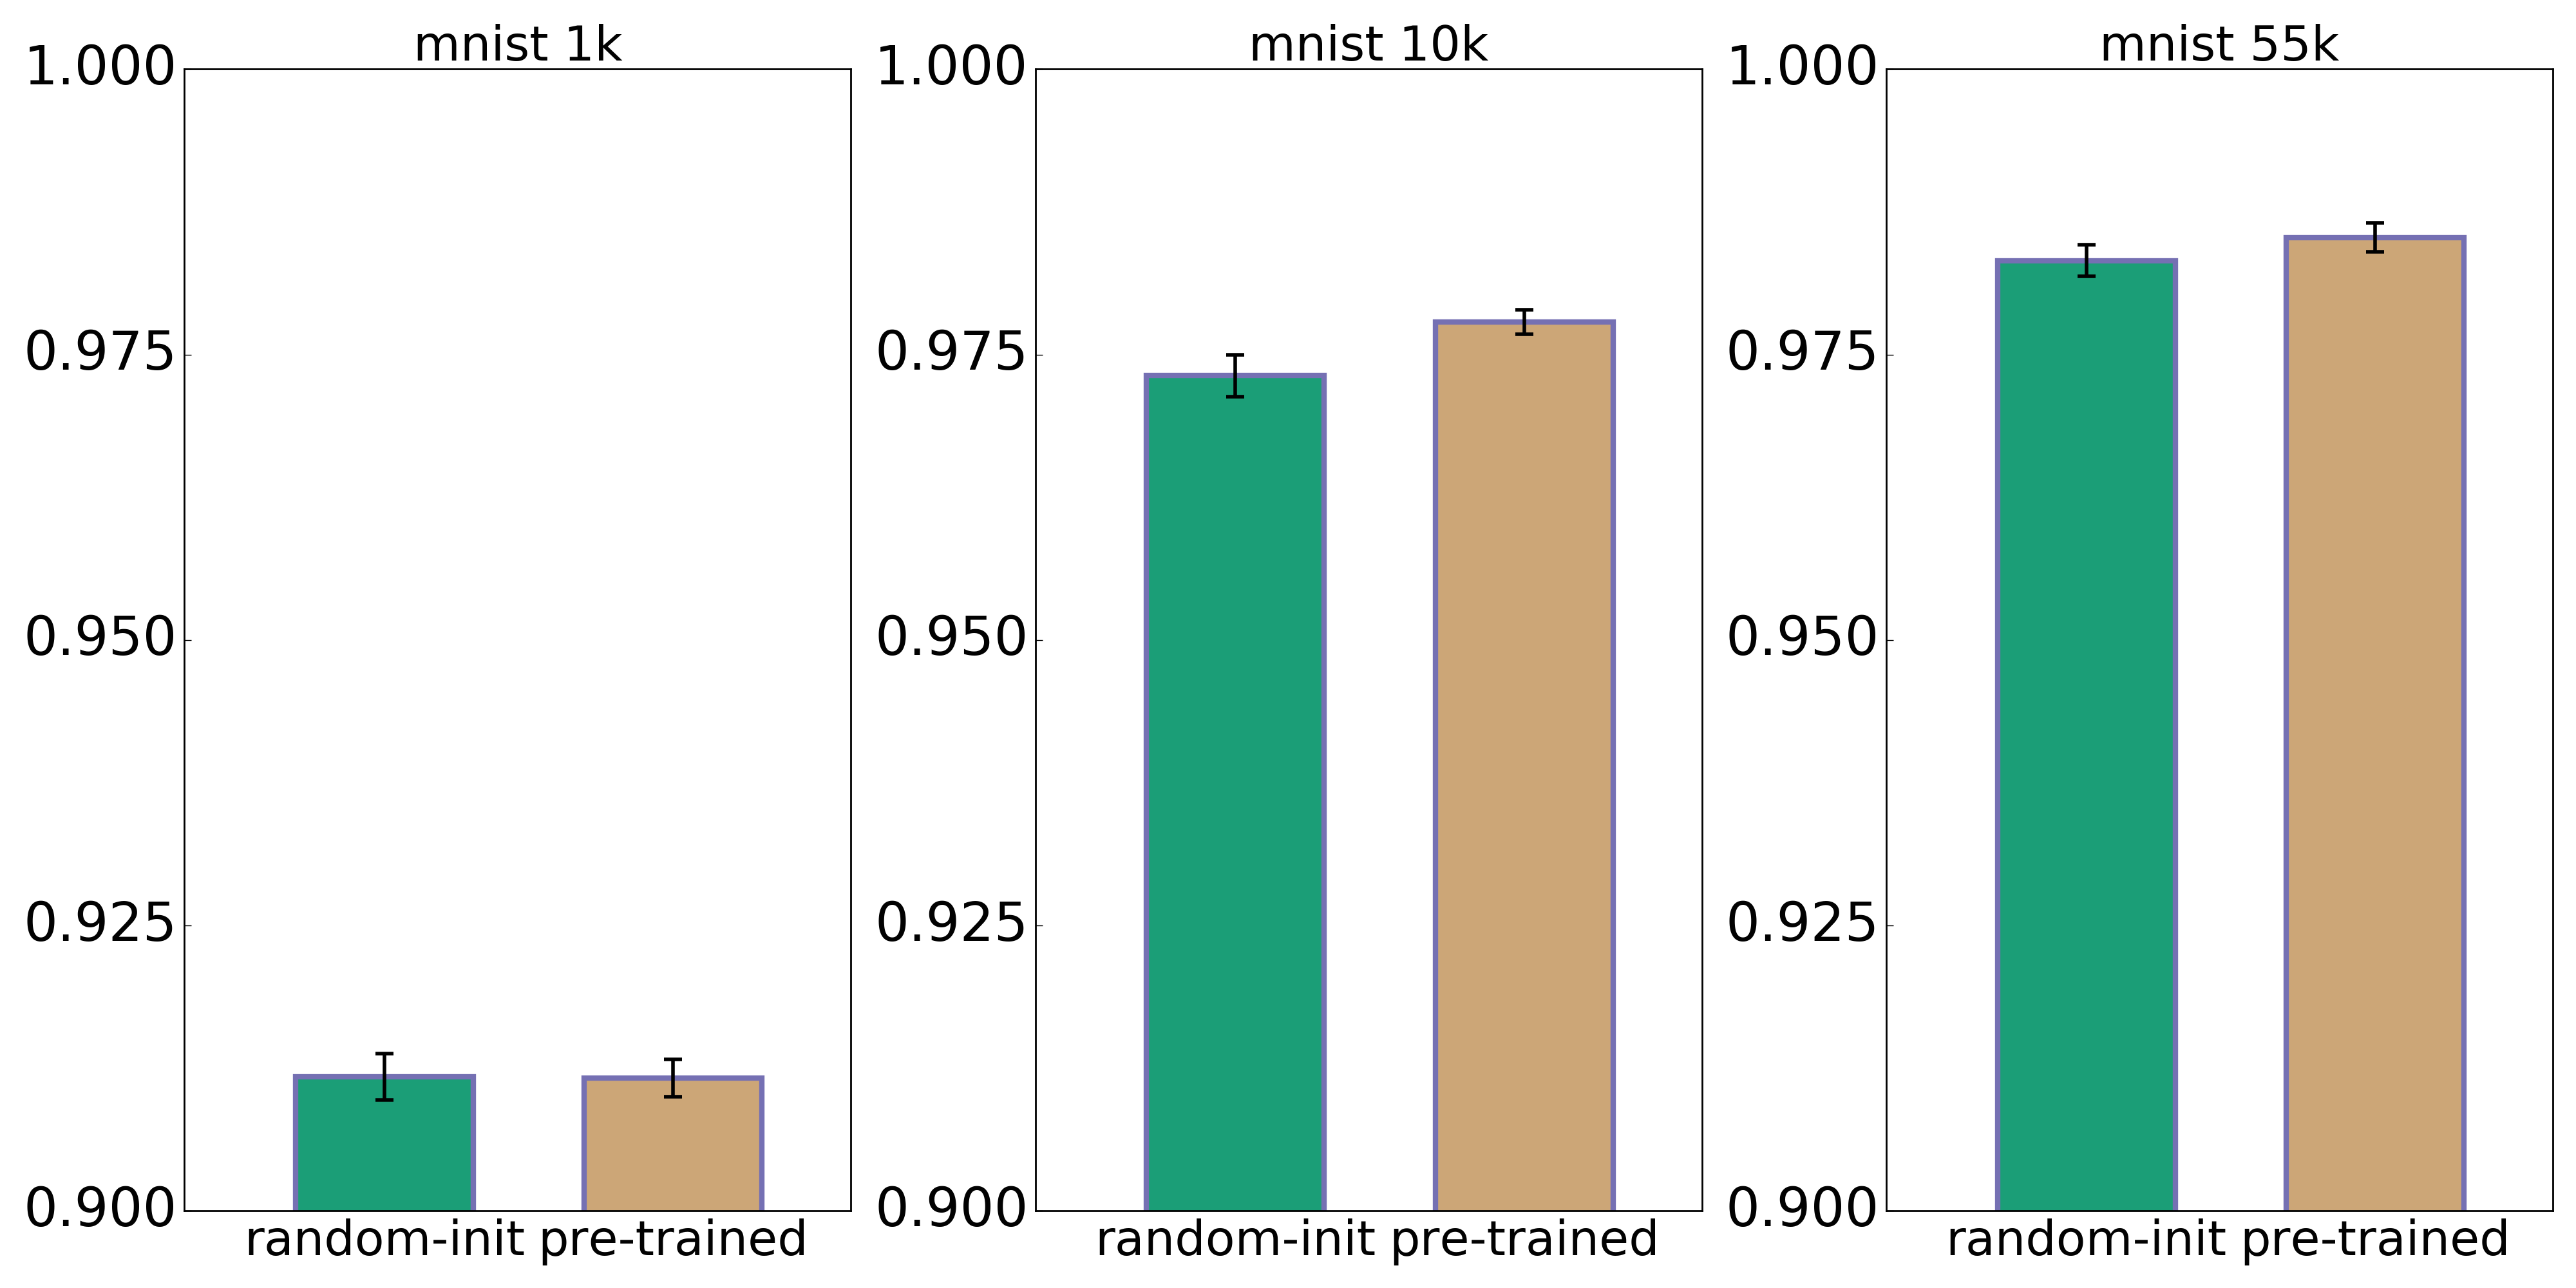
\includegraphics[width=\linewidth]{box_plots/boxplots_mnist.png}
	\caption{\emph{MNIST}: test set accuracy comparison for different training set sizes (stddev in black)}
	\label{fig:mnist_plot}
	\end{figure}

	\end{block}
	\end{column}
	\begin{column}{0.9\onecolwid}
	\begin{block}{}
	\emph{Experimental results:}

	\begin{figure}
	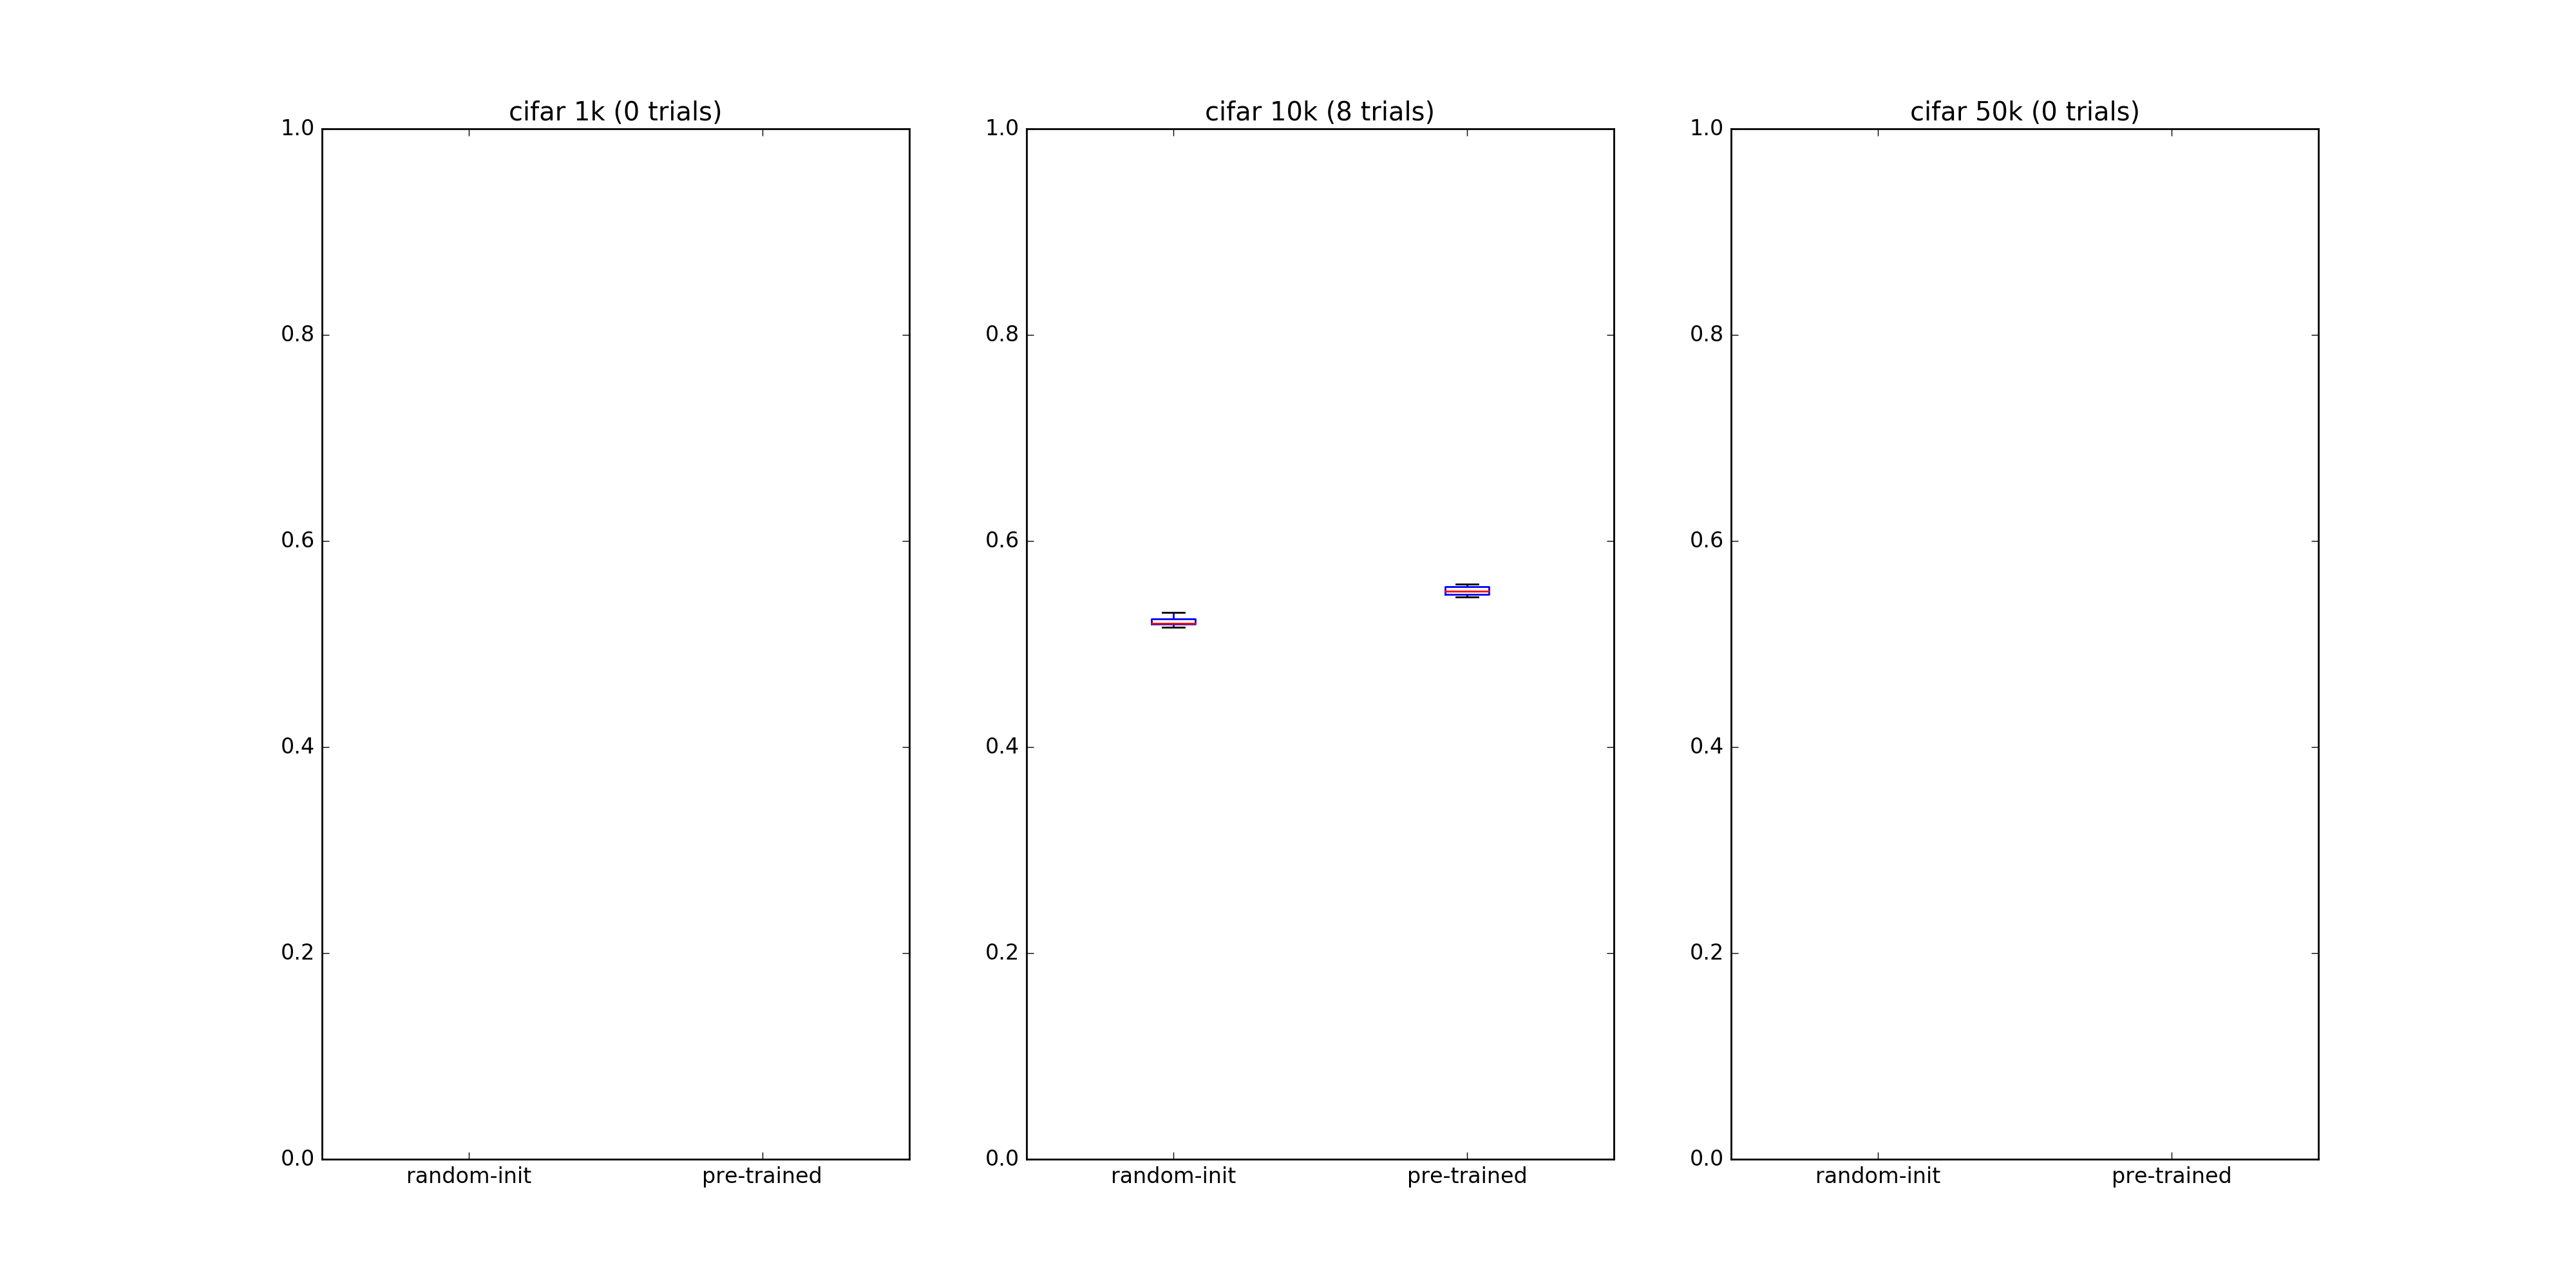
\includegraphics[width=\linewidth]{box_plots/boxplots_cifar.png}
	\caption{\emph{CIFAR-10}: test set accuracy comparison for different training set sizes (stddev in black)}
	\label{fig:cifar_plot}
	\end{figure}

	\end{block}
	\end{column}

	\begin{column}{0.9\onecolwid}
	\begin{block}{}
	\emph{Experimental results:}

	\begin{figure}
	\centering
	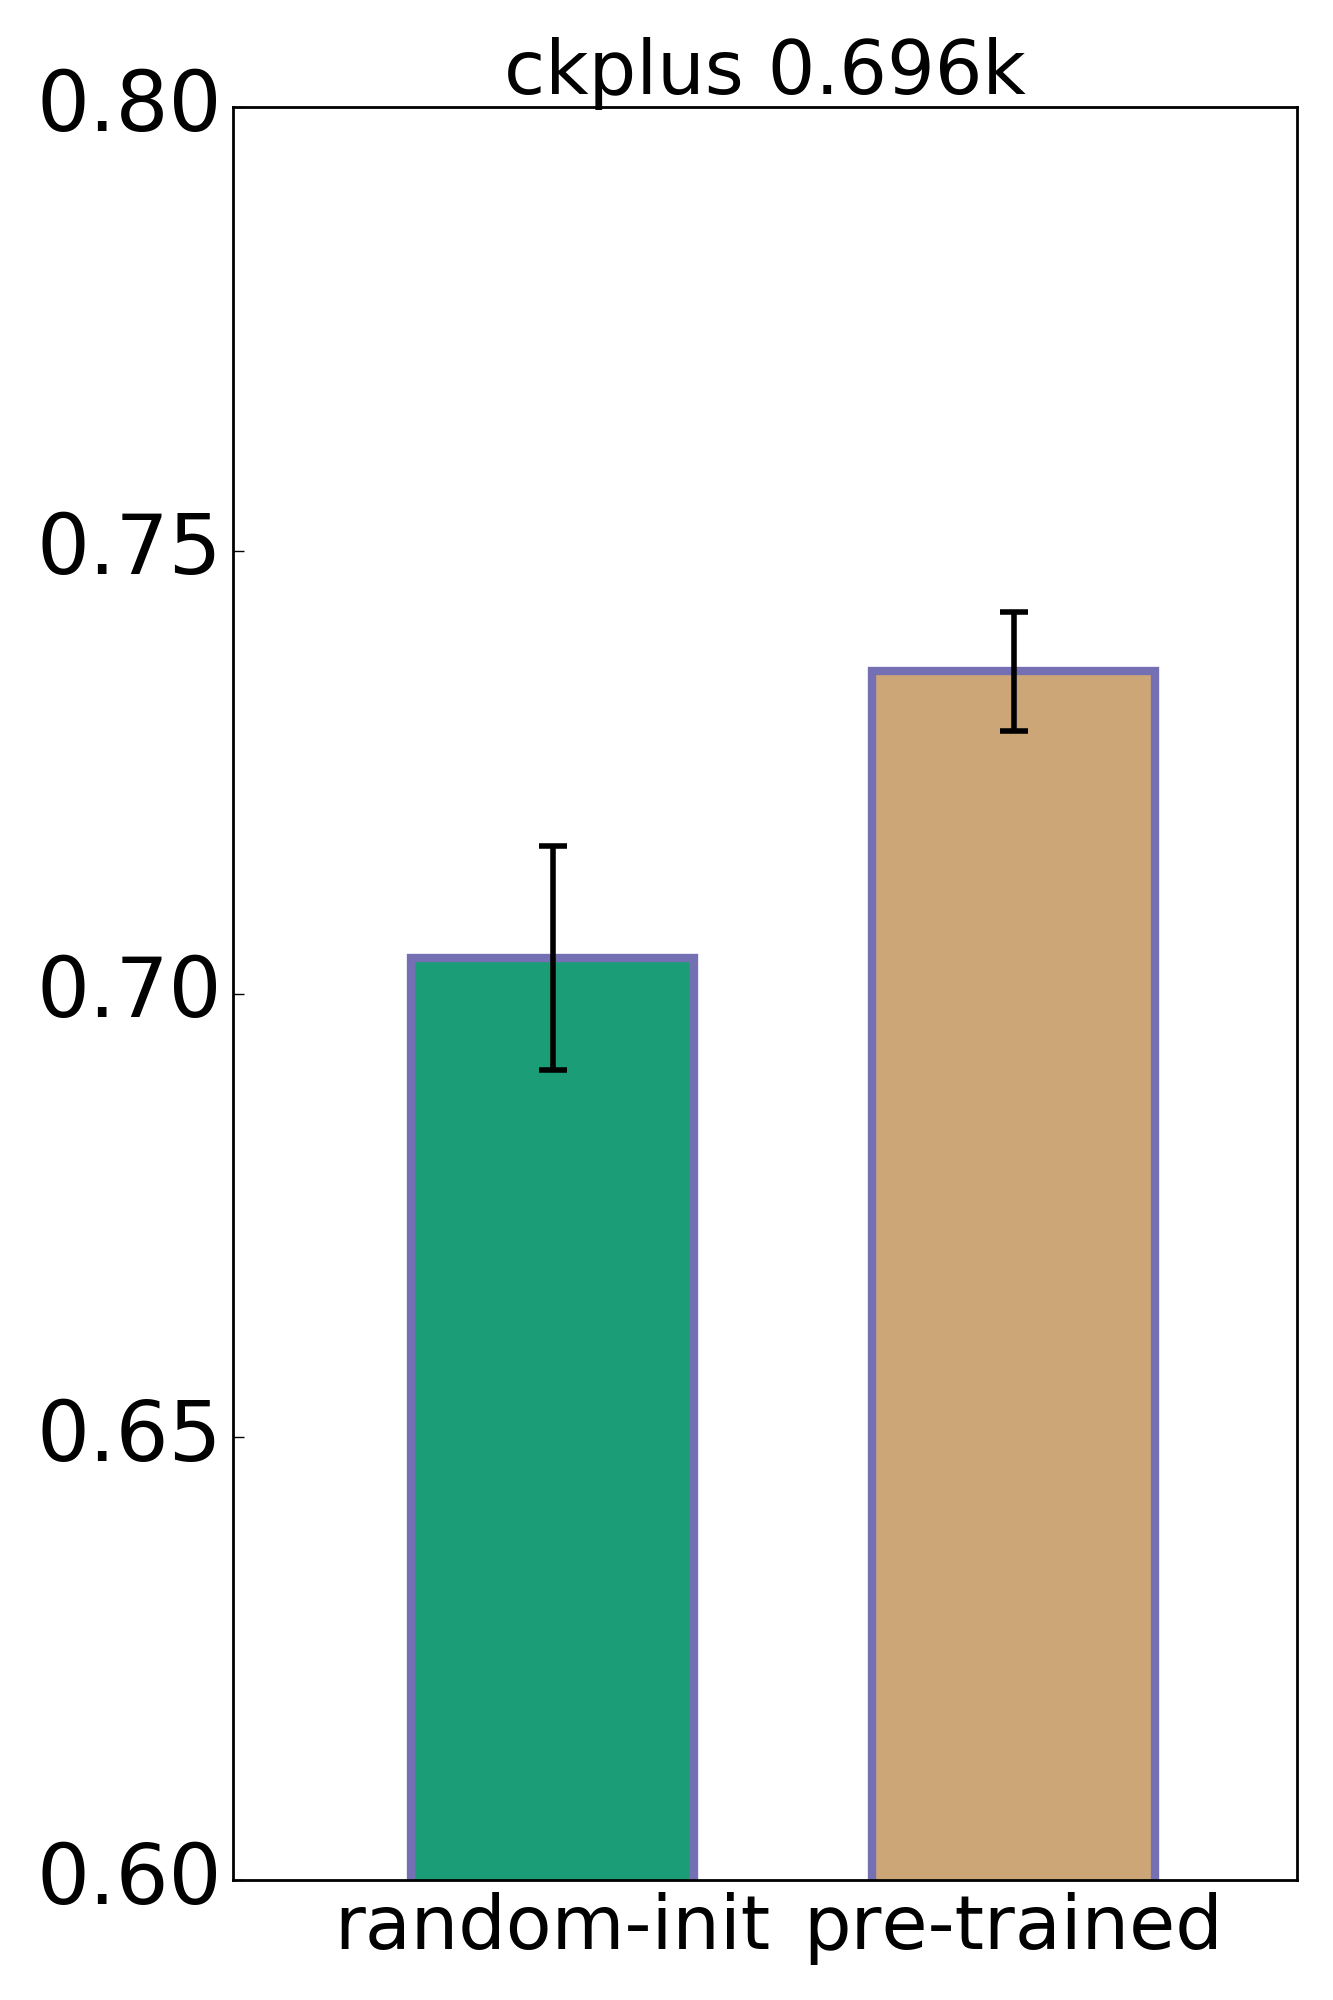
\includegraphics[width=0.33\linewidth]{box_plots/boxplots_ckplus.png}
	\caption{\emph{CK+}: test set accuracy comparison for 696 training images (stddev in black)}
	\label{fig:ckplus_plot}
	\end{figure}

	\end{block}


	\setbeamercolor{block title}{fg=ngreen,bg=white} % Colors of the block titles
	\setbeamercolor{block body}{fg=black,bg=white} % Colors of the body of blocks
	\setbeamercolor{block alerted title}{fg=black, bg=gray} % Colors of the highlighted block titles
	\setbeamercolor{block alerted body}{fg=black, bg=white} % Colors of the body of highlighted blocks
	% Many more colors are available for use in beamerthemeconfposter.sty

	\end{column}
\end{columns}


\end{alertblock}

\begin{alertblock} %{Conclusions}

\begin{columns}[t]

	\begin{column}{1.5\onecolwid}

		\begin{block}{Conclusions}

			\begin{itemize}
				\item Pre-Training consistently increases accuracy over all tested datasets and most training sizes (figures~\ref{fig:mnist_plot},~\ref{fig:cifar_plot} and~\ref{fig:ckplus_plot})

				\item After training, pre-trained network's first-layer filters show a clearer structure (figure~\ref{fig:cifar_filters}))
				%The first-layer filters of the pre-trained networks show a clear and interpretable structure as opposed to the ones learned by the randomly initialized network (\ref{fig:cifar_filters})

				\item When changing from sigmoidal to ReLU activation function, max-pooling no longer seems sufficient for CAE regularization (figure~\ref{fig:relu_cae}) 

				%ReLU's achieve very good reconstruction results but max-pooling does not seem sufficient for normalization. The learned filters lack a clear structure as can be seen in figure~\ref{fig:relu_cae}
			\end{itemize}

		\end{block}

	\end{column}

	\begin{column}{1.5\onecolwid}



			\begin{figure}
			\centering

				\begin{subfigure}{.4\linewidth}
					\centering
					
\includegraphics[width=0.1\linewidth]{graphics/cifar_filters/pre_trained_01.png} 
					
\includegraphics[width=0.1\linewidth]{graphics/cifar_filters/pre_trained_02.png} %\hspace{0.05\linewidth}
					
\includegraphics[width=0.1\linewidth]{graphics/cifar_filters/pre_trained_03.png}
					
\includegraphics[width=0.1\linewidth]{graphics/cifar_filters/pre_trained_04.png} %\hspace{0.05\linewidth}
					
\includegraphics[width=0.1\linewidth]{graphics/cifar_filters/pre_trained_05.png} %\hspace{0.05\linewidth}
					
\includegraphics[width=0.1\linewidth]{graphics/cifar_filters/pre_trained_06.png} \\
					
\includegraphics[width=0.1\linewidth]{graphics/cifar_filters/pre_trained_07.png} %\hspace{0.05\linewidth}
					
\includegraphics[width=0.1\linewidth]{graphics/cifar_filters/pre_trained_08.png} %\hspace{0.05\linewidth}
					
\includegraphics[width=0.1\linewidth]{graphics/cifar_filters/pre_trained_09.png}
					
\includegraphics[width=0.1\linewidth]{graphics/cifar_filters/pre_trained_10.png} 
					
\includegraphics[width=0.1\linewidth]{graphics/cifar_filters/pre_trained_11.png} %\hspace{0.05\linewidth}
					
\includegraphics[width=0.1\linewidth]{graphics/cifar_filters/pre_trained_12.png} \\
					
\includegraphics[width=0.1\linewidth]{graphics/cifar_filters/pre_trained_13.png} %\hspace{0.05\linewidth}
					
\includegraphics[width=0.1\linewidth]{graphics/cifar_filters/pre_trained_14.png} %\hspace{0.05\linewidth}
					
\includegraphics[width=0.1\linewidth]{graphics/cifar_filters/pre_trained_15.png}
					
\includegraphics[width=0.1\linewidth]{graphics/cifar_filters/pre_trained_16.png} %\hspace{0.05\linewidth}
					
\includegraphics[width=0.1\linewidth]{graphics/cifar_filters/pre_trained_17.png} %\hspace{0.05\linewidth}
					
\includegraphics[width=0.1\linewidth]{graphics/cifar_filters/pre_trained_18.png}
					%\caption{\emph{CIFAR-10}(CNN): random first layer filters, pre-trained}
				\end{subfigure}
				\begin{subfigure}{.4\linewidth}
					\centering
					
\includegraphics[width=0.1\linewidth]{graphics/cifar_filters/random_01.png} 
					
\includegraphics[width=0.1\linewidth]{graphics/cifar_filters/random_02.png} %\hspace{0.05\linewidth}
					
\includegraphics[width=0.1\linewidth]{graphics/cifar_filters/random_03.png}
					
\includegraphics[width=0.1\linewidth]{graphics/cifar_filters/random_04.png} %\hspace{0.05\linewidth}
					
\includegraphics[width=0.1\linewidth]{graphics/cifar_filters/random_05.png} %\hspace{0.05\linewidth}
					
\includegraphics[width=0.1\linewidth]{graphics/cifar_filters/random_06.png} \\
					\includegraphics[width=0.1\linewidth]{graphics/cifar_filters/random_07.png} %\hspace{0.05\linewidth}
					\includegraphics[width=0.1\linewidth]{graphics/cifar_filters/random_08.png} %\hspace{0.05\linewidth}
					\includegraphics[width=0.1\linewidth]{graphics/cifar_filters/random_09.png}
					\includegraphics[width=0.1\linewidth]{graphics/cifar_filters/random_10.png} 
					\includegraphics[width=0.1\linewidth]{graphics/cifar_filters/random_11.png} %\hspace{0.05\linewidth}
					\includegraphics[width=0.1\linewidth]{graphics/cifar_filters/random_12.png} \\
					\includegraphics[width=0.1\linewidth]{graphics/cifar_filters/random_13.png} %\hspace{0.05\linewidth}
					\includegraphics[width=0.1\linewidth]{graphics/cifar_filters/random_14.png} %\hspace{0.05\linewidth}
					\includegraphics[width=0.1\linewidth]{graphics/cifar_filters/random_15.png}
					\includegraphics[width=0.1\linewidth]{graphics/cifar_filters/random_16.png} %\hspace{0.05\linewidth}
					\includegraphics[width=0.1\linewidth]{graphics/cifar_filters/random_17.png} %\hspace{0.05\linewidth}
					\includegraphics[width=0.1\linewidth]{graphics/cifar_filters/random_18.png}
					%\caption{\emph{CIFAR-10}(CNN): random first layer filters, random-init}
				\end{subfigure}

			\caption{(\emph{CIFAR-10} CNN): Selection of first layer filters. pre-trained (left), random-init (right)}
			\label{fig:cifar_filters}

			\end{figure}

			\begin{figure}

				\begin{subfigure}{0.4\linewidth}

					\centering
					\includegraphics[width=0.4\linewidth]{graphics/reconstructions/cifar/relu/input_00_relu.png}
					\includegraphics[width=0.4\linewidth]{graphics/reconstructions/cifar/relu/reconstruction_00_relu.png}
					%\caption{(CAE:) Reconstruction example using ReLU activation + smaller network size}

				\end{subfigure}
				\begin{subfigure}{0.4\linewidth}

					\centering
					\includegraphics[width=0.1\linewidth]{graphics/reconstructions/cifar/relu/relu_filter_00.png} \hspace{0.05\linewidth}
					\includegraphics[width=0.1\linewidth]{graphics/reconstructions/cifar/relu/relu_filter_01.png} \hspace{0.05\linewidth}
					\includegraphics[width=0.1\linewidth]{graphics/reconstructions/cifar/relu/relu_filter_02.png} \\
					\vspace{0.05\linewidth}
					\includegraphics[width=0.1\linewidth]{graphics/reconstructions/cifar/relu/relu_filter_03.png} \hspace{0.05\linewidth}
					\includegraphics[width=0.1\linewidth]{graphics/reconstructions/cifar/relu/relu_filter_04.png} \hspace{0.05\linewidth}
					\includegraphics[width=0.1\linewidth]{graphics/reconstructions/cifar/relu/relu_filter_05.png} \\
					\vspace{0.05\linewidth}
					\includegraphics[width=0.1\linewidth]{graphics/reconstructions/cifar/relu/relu_filter_06.png} \hspace{0.05\linewidth}
					\includegraphics[width=0.1\linewidth]{graphics/reconstructions/cifar/relu/relu_filter_07.png} \hspace{0.05\linewidth}
					\includegraphics[width=0.1\linewidth]{graphics/reconstructions/cifar/relu/relu_filter_08.png} 

					%\caption{(CAE:) Structureless first layer filters learned by ReLU autoencoder}

				\end{subfigure}

			\caption{(ReLU CAE:) example input + reconstruction (left), selection of first layer filters (right) }
			\label{fig:relu_cae}

			\end{figure}
		
		\end{column}



\end{columns}

\end{alertblock}


\end{column}
\end{columns} % End of all the columns in the poster


\end{frame} % End of the enclosing frame

\end{document}
